\subsection{Mallob Integration}
- how we integrated CrowdHTN with Mallob
- this is done by implementing a job interface in Mallob
- the interface code can be found online in the Mallob repository \footnote{https://github.com/domschrei/mallob}
- and additionally a function to read an instance
- give a short overview of the interface
- a job is internally implemented as a state machine
- the state diagram is found at \ref{figure: mallob state diagram}
- from \cite{schreiber2021scalable} we know that Mallob aims to deliver latencies in the millisecond range

\begin{algorithm}
	\caption{The Mallob job interface}
	void appl\_start()\;
	void appl\_suspend()\;
	void appl\_resume()\;
	void appl\_terminate()\;
	void appl\_solved()\;
	JobResult appl\_getResult()\;
	void appl\_communicate()\;
	void appl\_communicate(source, mpi\_tag, message)\;
	void appl\_memoryPanic()\;
\end{algorithm}

\paragraph{Achieving millisecond latencies}
- big operations are put into separate threads
- this includes the \textit{start} function where the instance gets parsed and the CrowdHTN worker is initialized
- similarly, the CrowdHTN worker is put into a separate thread which is started in \textit{start}
- the functions \textit{suspend}, \textit{terminate} communicate with the CrowdHTN worker via atomics
- \textit{resume} is realized via a condition variable to wake up the worker thread
- where needed, locking is kept to an absolute minimum: messages are communicated from and to the CrowdHTN worker via dynamic arrays (realized through \textit{std::vector}) which are locked only for swapping the metadata in and out
- 

\paragraph{Handling version increases}
- false positives in loop detection necessitate restarts \ref{improv: loop detection}
- as a result, we need to invalidate all workers and start anew
-

\begin{figure}
	\caption{State transition diagram of a Mallob job}
	\label{figure: mallob state diagram}
	\centering
	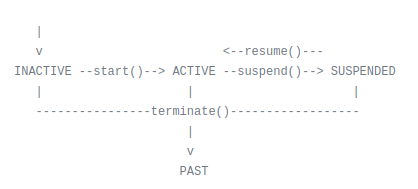
\includegraphics{images/prelim/mallob_state_diagram}
\end{figure}